\documentclass[12pt]{article}

\usepackage{sbc-template}
\usepackage{graphicx,url}
\usepackage[utf8]{inputenc}
\usepackage[T1]{fontenc}
\usepackage[brazil,english]{babel}
\usepackage{array}
\usepackage{booktabs}
\usepackage{listings}
\usepackage{xcolor}
\usepackage{float}

\sloppy

\definecolor{codegray}{rgb}{0.95,0.95,0.95}
\definecolor{codeblue}{rgb}{0.08,0.25,0.45}
\lstdefinestyle{codigo}{
  backgroundcolor=\color{codegray},
  basicstyle=\ttfamily\footnotesize,
  breaklines=true,
  frame=single,
  rulecolor=\color{black!20},
  keywordstyle=\color{codeblue}\bfseries,
  commentstyle=\color{black!55},
  stringstyle=\color{purple!70!black},
  showstringspaces=false,
  tabsize=2
}
\lstset{style=codigo}

\title{Pokedex em Grafos: Desenvolvimento de uma Aplicação Web com API REST, Autenticação JWT e Persistência em Neo4j}

\author{
Kaique Vinícius Oliveira Alves\inst{1},
Pedro Gabriel Mendes de Oliveira\inst{1},
Gustavo Borges Sousa\inst{1},\\
Peterson Silva Ribeiro\inst{1},
Matheus Henrique do Couto\inst{1}
}

\address{
Banco de Dados II -- Universidade Estadual de Goiás (UEG)\\
\email{\{kaique.alves, pedro.mendes, gustavo.borges, peterson.ribeiro, matheus.couto\}@discente.ueg.br}
}

\begin{document}

\maketitle

\begin{abstract}
This paper presents the development of a web-based graph Pokedex, integrating a pure HTML, CSS and JavaScript front-end with a REST API built with Node.js and Express. The system models Pokemon, types, skills, weaknesses, evolutions, users, favorites and teams as nodes and relationships in Neo4j. It also implements JWT authentication, bcrypt password hashing, route protection, input validation, centralized error handling and Docker-based deployment. The results indicate that graph modeling improves the representation of semantic relationships in the domain and supports interactive queries over the application data.
\end{abstract}

\begin{resumo}
Este artigo apresenta o desenvolvimento de uma Pokedex em Grafos, integrando um front-end em HTML, CSS e JavaScript puro com uma API REST em Node.js e Express. O sistema modela Pokémon, tipos, habilidades, fraquezas, evoluções, usuários, favoritos e equipes como nós e relacionamentos no Neo4j. Também são implementados autenticação JWT, hash de senhas com bcrypt, proteção de rotas, validação de entrada, tratamento centralizado de erros e execução com Docker. Os resultados indicam que a modelagem em grafo favorece a representação das relações semânticas do domínio e apoia consultas interativas sobre os dados da aplicação.
\end{resumo}

\section{Introdução}

No universo da franquia Pokémon, uma Pokedex é um dispositivo ou catálogo digital utilizado para registrar, consultar e organizar informações sobre criaturas chamadas Pokémon. De forma geral, ela funciona como uma enciclopédia: cada registro contém dados como nome, número, imagem, descrição, tipo, habilidades e informações de evolução. Para jogadores e usuários familiarizados com esse universo, a Pokedex serve como uma ferramenta de consulta rápida para comparar criaturas, entender suas características e acompanhar o progresso de uma coleção.

Embora o termo Pokedex esteja fortemente associado ao mundo Pokémon, sua ideia central é próxima de muitos sistemas de informação: organizar entidades, atributos e relações de forma acessível ao usuário. Uma Pokedex digital pode, portanto, ser entendida como um catálogo interativo no qual cada Pokémon é um recurso principal e suas conexões com outros elementos, como tipos, fraquezas, habilidades e evoluções, enriquecem a experiência de consulta. Essa característica torna o domínio adequado para explorar conceitos de banco de dados, APIs REST, autenticação e modelagem de relacionamentos.

Este trabalho apresenta o desenvolvimento de uma Pokedex em Grafos. Diferentemente de uma Pokedex simples, baseada apenas em uma lista estática de registros, a aplicação desenvolvida representa os dados como um conjunto de nós e relacionamentos no banco Neo4j. Assim, um Pokémon não é apenas um item isolado; ele se relaciona com tipos, possui fraquezas, pode evoluir para outro Pokémon, possuir habilidades, ser favoritado por usuários e compor equipes de treinadores.

A aplicação foi construída com front-end em HTML, CSS e JavaScript puro, consumindo uma API REST desenvolvida em Node.js com Express. A persistência dos dados foi implementada com Neo4j, enquanto a autenticação utiliza JSON Web Tokens (JWT) e bcrypt para armazenamento seguro de senhas. Além disso, o ambiente foi preparado com Docker e Docker Compose, permitindo a execução da aplicação e do banco em containers separados.

O restante deste artigo está organizado da seguinte forma. A Seção 2 contextualiza o problema e apresenta a justificativa do projeto. A Seção 3 descreve os objetivos. A Seção 4 apresenta a fundamentação teórica. A Seção 5 discute a metodologia. A Seção 6 descreve a modelagem dos dados. A Seção 7 apresenta a implementação. A Seção 8 relata os resultados obtidos. Por fim, as Seções 9 e 10 apresentam discussão, conclusão e trabalhos futuros.

\section{Contextualização do Problema e Justificativa}

Sistemas de catálogo frequentemente começam como listas simples, mas muitos domínios reais exigem a representação de relações entre entidades. Em uma Pokedex, por exemplo, o usuário pode querer saber quais Pokémon pertencem a determinado tipo, quais possuem fraqueza contra outro tipo, quais evoluem para determinada forma ou quais fazem parte de uma equipe. Quando tais conexões passam a ser importantes, a modelagem deixa de ser apenas uma questão de cadastro e passa a envolver a representação de dependências, ligações e padrões.

Uma abordagem relacional tradicional poderia representar essas conexões por tabelas e chaves estrangeiras. No entanto, esse tipo de modelagem tende a exigir tabelas intermediárias para relações muitos-para-muitos, além de consultas com múltiplas junções para recuperar uma visão completa de um recurso. Como o domínio escolhido possui forte natureza relacional, optou-se por utilizar um banco de dados em grafo. Nessa abordagem, entidades são representadas como nós e suas conexões como arestas, o que torna a estrutura mais próxima da linguagem natural do problema.

A justificativa pedagógica do projeto está relacionada à integração de diferentes conteúdos de desenvolvimento back-end e banco de dados. O sistema reúne API REST, autenticação, validação, tratamento de erros, persistência, consumo de API pelo front-end e conteinerização. Além disso, o tema escolhido é suficientemente rico para demonstrar relacionamentos entre recursos, operações CRUD e uso prático de um banco orientado a grafos.

\section{Objetivos}

O objetivo geral do trabalho é desenvolver uma aplicação web completa para consulta e gerenciamento de uma Pokedex em Grafos, integrando front-end, API REST, autenticação e persistência em Neo4j.

Como objetivos específicos, destacam-se:

\begin{itemize}
  \item explicar e representar o conceito de Pokedex para usuários familiarizados ou não com Pokémon;
  \item implementar uma API REST em Node.js com Express;
  \item modelar Pokémon, tipos, habilidades, fraquezas, evoluções, usuários, favoritos e equipes no Neo4j;
  \item implementar autenticação com JWT e hash de senhas com bcrypt;
  \item proteger rotas que exigem login;
  \item validar dados de entrada em rotas de cadastro e atualização;
  \item criar tratamento centralizado de erros e middleware de log;
  \item desenvolver front-end em HTML, CSS e JavaScript puro consumindo a API;
  \item disponibilizar o ambiente com Docker e Docker Compose.
\end{itemize}

\section{Fundamentação Teórica}

\subsection{APIs REST e Express}

Uma API REST organiza a comunicação entre cliente e servidor por meio de recursos acessados com métodos HTTP, como GET, POST, PUT e DELETE. No projeto, essa arquitetura foi utilizada para expor recursos como Pokémon, tipos, autenticação, favoritos e equipes. O Express foi escolhido por ser um framework minimalista para Node.js, amplamente usado na criação de aplicações web e APIs \cite{expressDocs}.

No contexto do sistema, o front-end não acessa diretamente o banco de dados. Ele envia requisições HTTP para a API, que valida dados, executa consultas no Neo4j e devolve respostas em JSON. Essa separação facilita a organização do código e permite que o back-end concentre regras de negócio e segurança.

\subsection{Banco de Dados em Grafos e Neo4j}

Bancos de dados em grafos são adequados para domínios em que os relacionamentos são tão relevantes quanto os próprios dados. O Neo4j utiliza nós, relacionamentos e propriedades para representar informações \cite{neo4jDocs}. No projeto, Pokémon, usuários, tipos, equipes e habilidades são nós; já relações como \texttt{FAVORITOU}, \texttt{TEM\_TIPO} e \texttt{TEM\_MEMBRO} são arestas.

Essa modelagem torna consultas semânticas mais diretas. Por exemplo, em vez de consultar várias tabelas para descobrir os Pokémon de uma equipe, basta seguir as relações entre o nó da equipe e os nós de Pokémon.

\subsection{JWT e bcrypt}

JSON Web Token (JWT) é um padrão para representar informações de forma compacta e assinada entre partes \cite{jwtIntro}. Na aplicação, após o login, o servidor gera um token contendo o identificador e o e-mail do usuário. Esse token é enviado pelo front-end em requisições protegidas.

O bcrypt é utilizado para proteger senhas antes de armazená-las \cite{bcryptPackage}. Em vez de salvar a senha em texto puro, a aplicação salva um hash. Durante o login, a senha informada é comparada com esse hash, sem necessidade de recuperar a senha original.

\subsection{Docker}

Docker permite empacotar aplicações e suas dependências em containers, criando ambientes reproduzíveis \cite{dockerDocs}. No projeto, Docker Compose foi utilizado para orquestrar dois serviços principais: o serviço da aplicação e o serviço do banco Neo4j. A comunicação entre eles ocorre por uma rede Docker personalizada, enquanto os dados do banco são persistidos por volumes.

\section{Metodologia}

A metodologia adotada seguiu uma abordagem incremental. Inicialmente, definiu-se o domínio da aplicação e os recursos principais. Em seguida, foi projetado o modelo de dados em grafo, considerando os nós e relacionamentos necessários para representar a Pokedex. Após essa etapa, foi implementada a API REST em Node.js com Express, seguida pela criação do front-end em HTML, CSS e JavaScript puro.

O desenvolvimento do back-end foi organizado em rotas, controllers, middlewares e camada de banco. As rotas recebem as requisições HTTP; os controllers implementam a lógica de negócio; os middlewares tratam autenticação, validação, logs e erros; e o arquivo de banco centraliza a conexão com o Neo4j.

Por fim, o ambiente foi conteinerizado com Docker. O Dockerfile define a imagem da aplicação, enquanto o Docker Compose descreve os serviços, variáveis de ambiente, portas, volumes e rede. Testes manuais foram realizados no navegador, no terminal e no Neo4j Browser para verificar o funcionamento do sistema.

\section{Descrição da Modelagem}

A modelagem do sistema foi baseada em nós e relacionamentos. A Figura \ref{fig:modelagem} apresenta uma visão textual da estrutura do grafo.

\begin{figure}[H]
\centering
\fbox{
\begin{minipage}{0.92\textwidth}
\small
\textbf{Nós principais:} Usuario, Pokemon, Tipo, Equipe, Habilidade.\\[2mm]
\textbf{Relacionamentos:}\\
(Usuario)-[:FAVORITOU]-\textgreater(Pokemon)\\
(Usuario)-[:CRIOU\_EQUIPE]-\textgreater(Equipe)\\
(Equipe)-[:TEM\_MEMBRO]-\textgreater(Pokemon)\\
(Pokemon)-[:TEM\_TIPO]-\textgreater(Tipo)\\
(Pokemon)-[:TEM\_FRAQUEZA]-\textgreater(Tipo)\\
(Pokemon)-[:TEM\_HABILIDADE]-\textgreater(Habilidade)\\
(Pokemon)-[:EVOLUI\_PARA]-\textgreater(Pokemon)
\end{minipage}
}
\caption{Modelo conceitual do grafo utilizado pela Pokedex.}
\label{fig:modelagem}
\end{figure}

O nó \texttt{Pokemon} possui propriedades como identificador, número, nome, descrição e URL da imagem. O nó \texttt{Tipo} possui nome e cor, permitindo classificar visualmente os Pokémon. O nó \texttt{Usuario} armazena nome, e-mail e hash da senha. O nó \texttt{Equipe} representa conjuntos criados por usuários, enquanto \texttt{Habilidade} descreve características especiais associadas a Pokémon.

A relação \texttt{FAVORITOU} indica que um usuário adicionou determinado Pokémon à sua lista de favoritos. A relação \texttt{CRIOU\_EQUIPE} liga o usuário a uma equipe, e \texttt{TEM\_MEMBRO} liga a equipe aos Pokémon selecionados. Relações como \texttt{TEM\_TIPO}, \texttt{TEM\_FRAQUEZA} e \texttt{EVOLUI\_PARA} representam aspectos próprios do domínio Pokémon.

\section{Implementação}

\subsection{Arquitetura Geral}

A arquitetura da aplicação é composta por três camadas principais. A primeira é o front-end, responsável pela interface do usuário. A segunda é o back-end, responsável pela API REST e pelas regras de negócio. A terceira é o banco Neo4j, responsável pela persistência dos dados em grafo.

\begin{figure}[H]
\centering
\fbox{
\begin{minipage}{0.88\textwidth}
\centering
\small
Navegador (HTML, CSS, JavaScript)\\
$\downarrow$ requisições HTTP com fetch\\
API REST Node.js + Express\\
$\downarrow$ consultas Cypher com neo4j-driver\\
Banco Neo4j (nós e relacionamentos)
\end{minipage}
}
\caption{Arquitetura geral da aplicação.}
\label{fig:arquitetura}
\end{figure}

\subsection{Conexão com o Neo4j}

A conexão com o banco é centralizada no arquivo \texttt{database.js}. O trecho a seguir mostra a criação do driver:

\begin{lstlisting}[language=JavaScript]
const driver = neo4j.driver(
  process.env.NEO4J_URI || 'bolt://localhost:7687',
  neo4j.auth.basic(
    process.env.NEO4J_USER || 'neo4j',
    process.env.NEO4J_PASSWORD || 'pokedex123'
  )
);
\end{lstlisting}

As funções \texttt{runRead} e \texttt{runWrite} separam consultas de leitura e escrita. Ambas abrem uma sessão, executam a transação e fecham a sessão no bloco \texttt{finally}, reduzindo o risco de conexões abertas.

\subsection{CRUD de Pokémon e Tipo}

O recurso Pokémon possui rotas para listar, buscar, criar, atualizar e remover registros. O mesmo ocorre com o recurso Tipo. O trecho a seguir exemplifica as rotas de Pokémon:

\begin{lstlisting}[language=JavaScript]
router.get('/', ctrl.listar);
router.get('/:id', ctrl.buscar);
router.post('/', auth, validarPokemon, ctrl.criar);
router.put('/:id', auth, validarPokemon, ctrl.atualizar);
router.delete('/:id', auth, ctrl.remover);
\end{lstlisting}

As rotas de criação, atualização e remoção são protegidas pelo middleware \texttt{auth}. Além disso, as rotas POST e PUT usam \texttt{validarPokemon}, garantindo que dados obrigatórios sejam enviados antes da execução da lógica do controller.

Na criação de Pokémon, o controller cria o nó e seus relacionamentos. O uso de Cypher permite declarar diretamente o padrão de grafo a ser persistido:

\begin{lstlisting}[language=SQL]
MATCH (tipo:Tipo {id: $tipoId})
MERGE (p:Pokemon {numero: $numero})
ON CREATE SET p.id = randomUUID(), p.createdAt = datetime()
SET p.nome = $nome,
    p.sprite_url = $sprite_url,
    p.descricao = $descricao,
    p.updatedAt = datetime()
MERGE (p)-[:TEM_TIPO]->(tipo)
\end{lstlisting}

\subsection{Autenticação e Proteção de Rotas}

O cadastro de usuário verifica se o e-mail já existe e gera o hash da senha:

\begin{lstlisting}[language=JavaScript]
const existentes = await runRead(
  'MATCH (u:Usuario {email: $email}) RETURN u LIMIT 1',
  { email }
);
if (existentes.length) {
  return res.status(409).json({ erro: 'E-mail ja cadastrado.' });
}

const senhaHash = await bcrypt.hash(senha, 10);
\end{lstlisting}

No login, a senha informada é comparada com o hash armazenado. Quando a comparação é válida, um token JWT é gerado:

\begin{lstlisting}[language=JavaScript]
const senhaCorreta = await bcrypt.compare(senha, usuario.senhaHash || '');
if (!senhaCorreta) {
  return res.status(401).json({ erro: 'E-mail ou senha invalidos.' });
}

const token = jwt.sign(
  { id: usuario.id, email: usuario.email },
  process.env.JWT_SECRET,
  { expiresIn: '8h' }
);
\end{lstlisting}

O middleware de autenticação verifica se o token foi enviado no cabeçalho da requisição:

\begin{lstlisting}[language=JavaScript]
if (!authHeader || !authHeader.startsWith('Bearer ')) {
  return res.status(401).json({ erro: 'Token nao fornecido.' });
}

const token = authHeader.split(' ')[1];
const payload = jwt.verify(token, process.env.JWT_SECRET);
req.usuarioId = payload.id;
next();
\end{lstlisting}

\subsection{Validação, Logs e Tratamento de Erros}

A validação impede que registros inválidos cheguem ao controller:

\begin{lstlisting}[language=JavaScript]
if (!nome || nome.trim() === '') erros.push('Campo "nome" e obrigatorio.');
if (!numero || Number.isNaN(Number(numero))) {
  erros.push('Campo "numero" deve ser numerico.');
}
if (!tipoId) erros.push('Campo "tipoId" e obrigatorio.');
\end{lstlisting}

O middleware de log registra método, URL, status e tempo de resposta:

\begin{lstlisting}[language=JavaScript]
res.on('finish', () => {
  const duracao = Date.now() - inicio;
  console.log(`${req.method} ${req.originalUrl} -> ${res.statusCode} (${duracao}ms)`);
});
\end{lstlisting}

O tratamento centralizado de erros padroniza as respostas:

\begin{lstlisting}[language=JavaScript]
function erroMiddleware(err, req, res, next) {
  const status = err.status || 500;
  const mensagem = err.message || 'Erro interno do servidor.';
  res.status(status).json({ erro: mensagem });
}
\end{lstlisting}

\subsection{Consumo da API pelo Front-end}

O front-end utiliza a API \texttt{fetch} para se comunicar com o back-end \cite{mdnFetch}. A função \texttt{api} centraliza as requisições:

\begin{lstlisting}[language=JavaScript]
async function api(path, options = {}) {
  const headers = { 'Content-Type': 'application/json', ...(options.headers || {}) };
  if (state.token) headers.Authorization = `Bearer ${state.token}`;

  const response = await fetch(`${API_URL}${path}`, { ...options, headers });
  const payload = await response.json().catch(() => ({}));

  if (!response.ok) {
    const details = payload.erro || payload.erros?.join(' ') || 'Falha na requisicao.';
    throw new Error(details);
  }
  return payload;
}
\end{lstlisting}

Após o login, o token é salvo no \texttt{localStorage}, permitindo manter a sessão durante a navegação:

\begin{lstlisting}[language=JavaScript]
localStorage.setItem('pokedexToken', state.token);
localStorage.setItem('pokedexUser', JSON.stringify(state.user));
\end{lstlisting}

\subsection{Ambiente Docker}

O Dockerfile utiliza uma construção em duas etapas: a primeira compila o front-end e a segunda prepara a aplicação Node.js para execução. O Docker Compose define dois serviços principais: \texttt{app} e \texttt{neo4j}. O serviço da aplicação se conecta ao banco pela URI \texttt{bolt://neo4j:7687}, usando o nome do serviço na rede Docker.

\section{Resultados Obtidos}

A aplicação foi executada localmente em ambiente Docker, com o serviço da aplicação publicado na porta 3000 e o Neo4j publicado nas portas 7474 e 7687. A Figura \ref{fig:interface} apresenta a interface da Pokedex em funcionamento.

\begin{figure}[H]
\centering
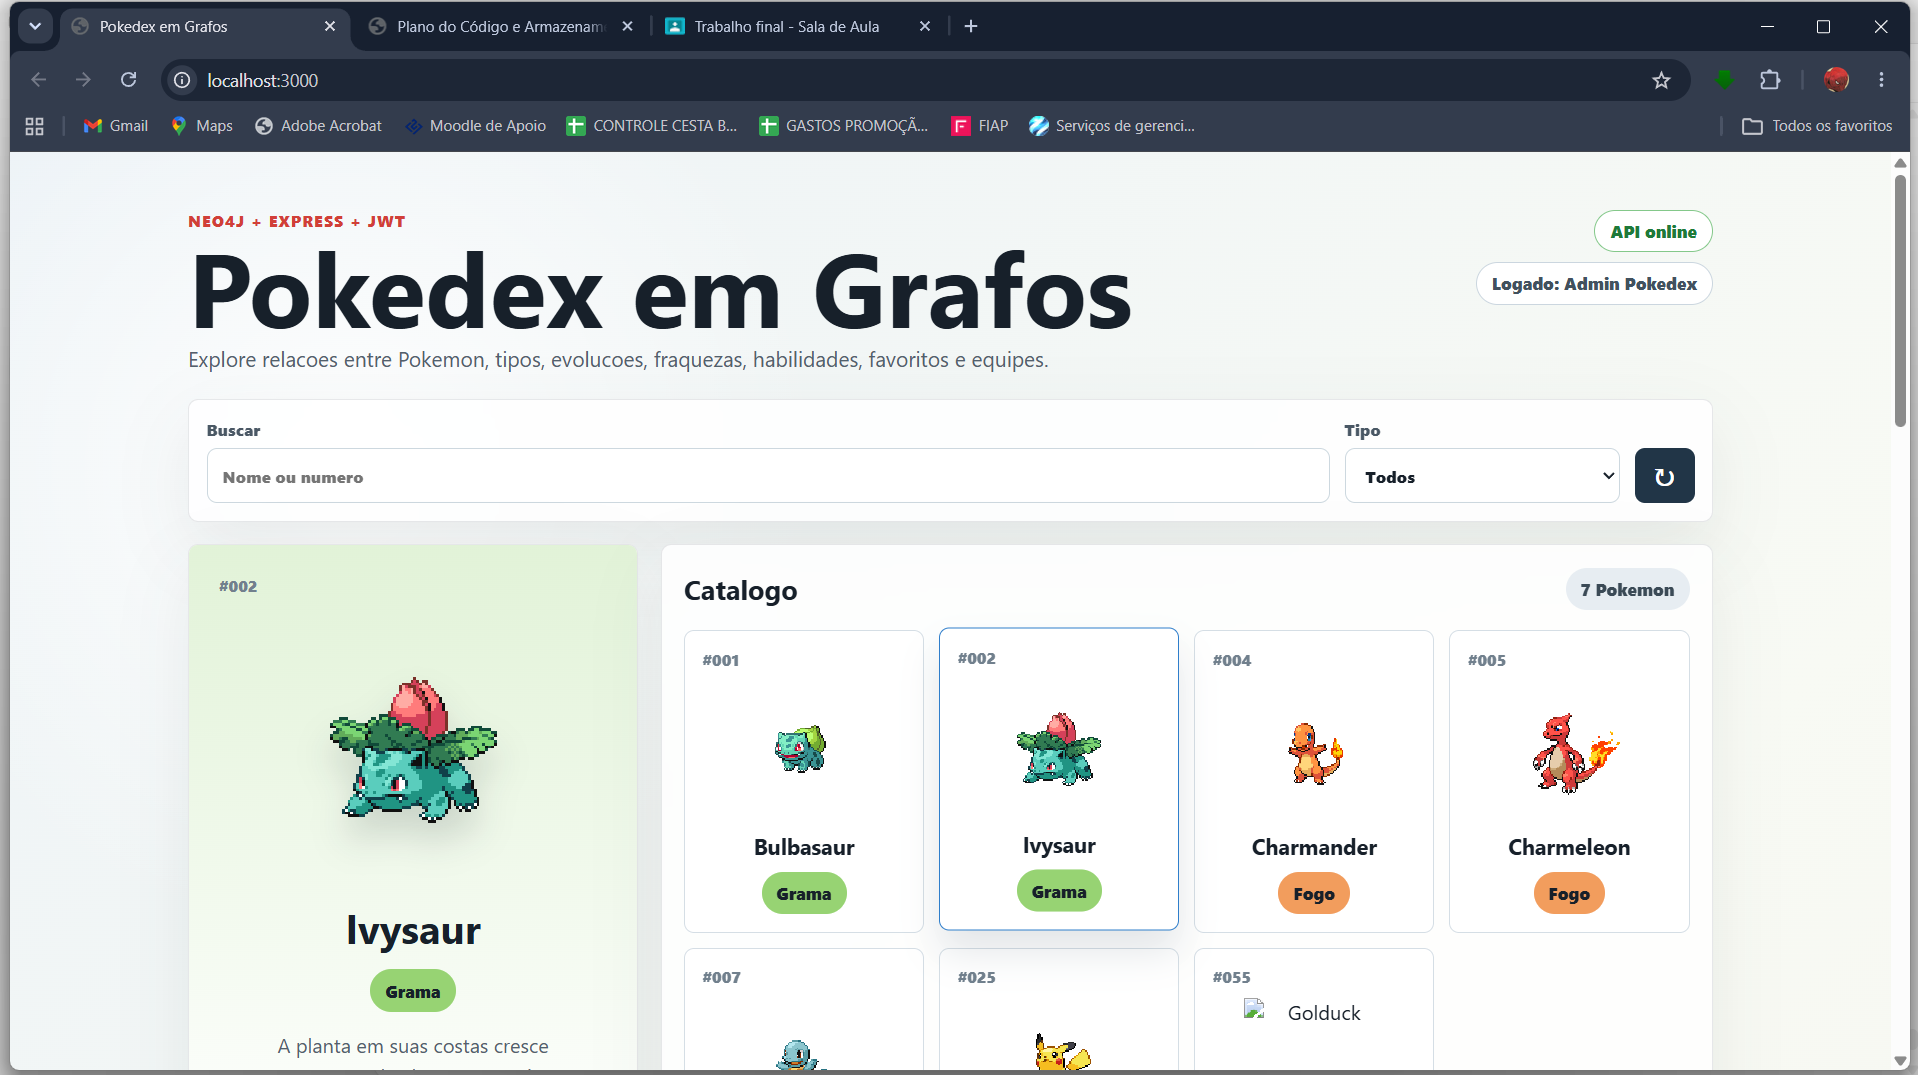
\includegraphics[width=.95\textwidth]{figuras/interface-pokedex.png}
\caption{Interface web da Pokedex em Grafos.}
\label{fig:interface}
\end{figure}

Na interface, foi possível consultar Pokémon, visualizar detalhes, filtrar por tipo, fazer login, cadastrar novos Pokémon, editar registros, remover Pokémon, favoritar e criar equipes. A Figura \ref{fig:neo4j} mostra o grafo consultado no Neo4j Browser.

\begin{figure}[H]
\centering
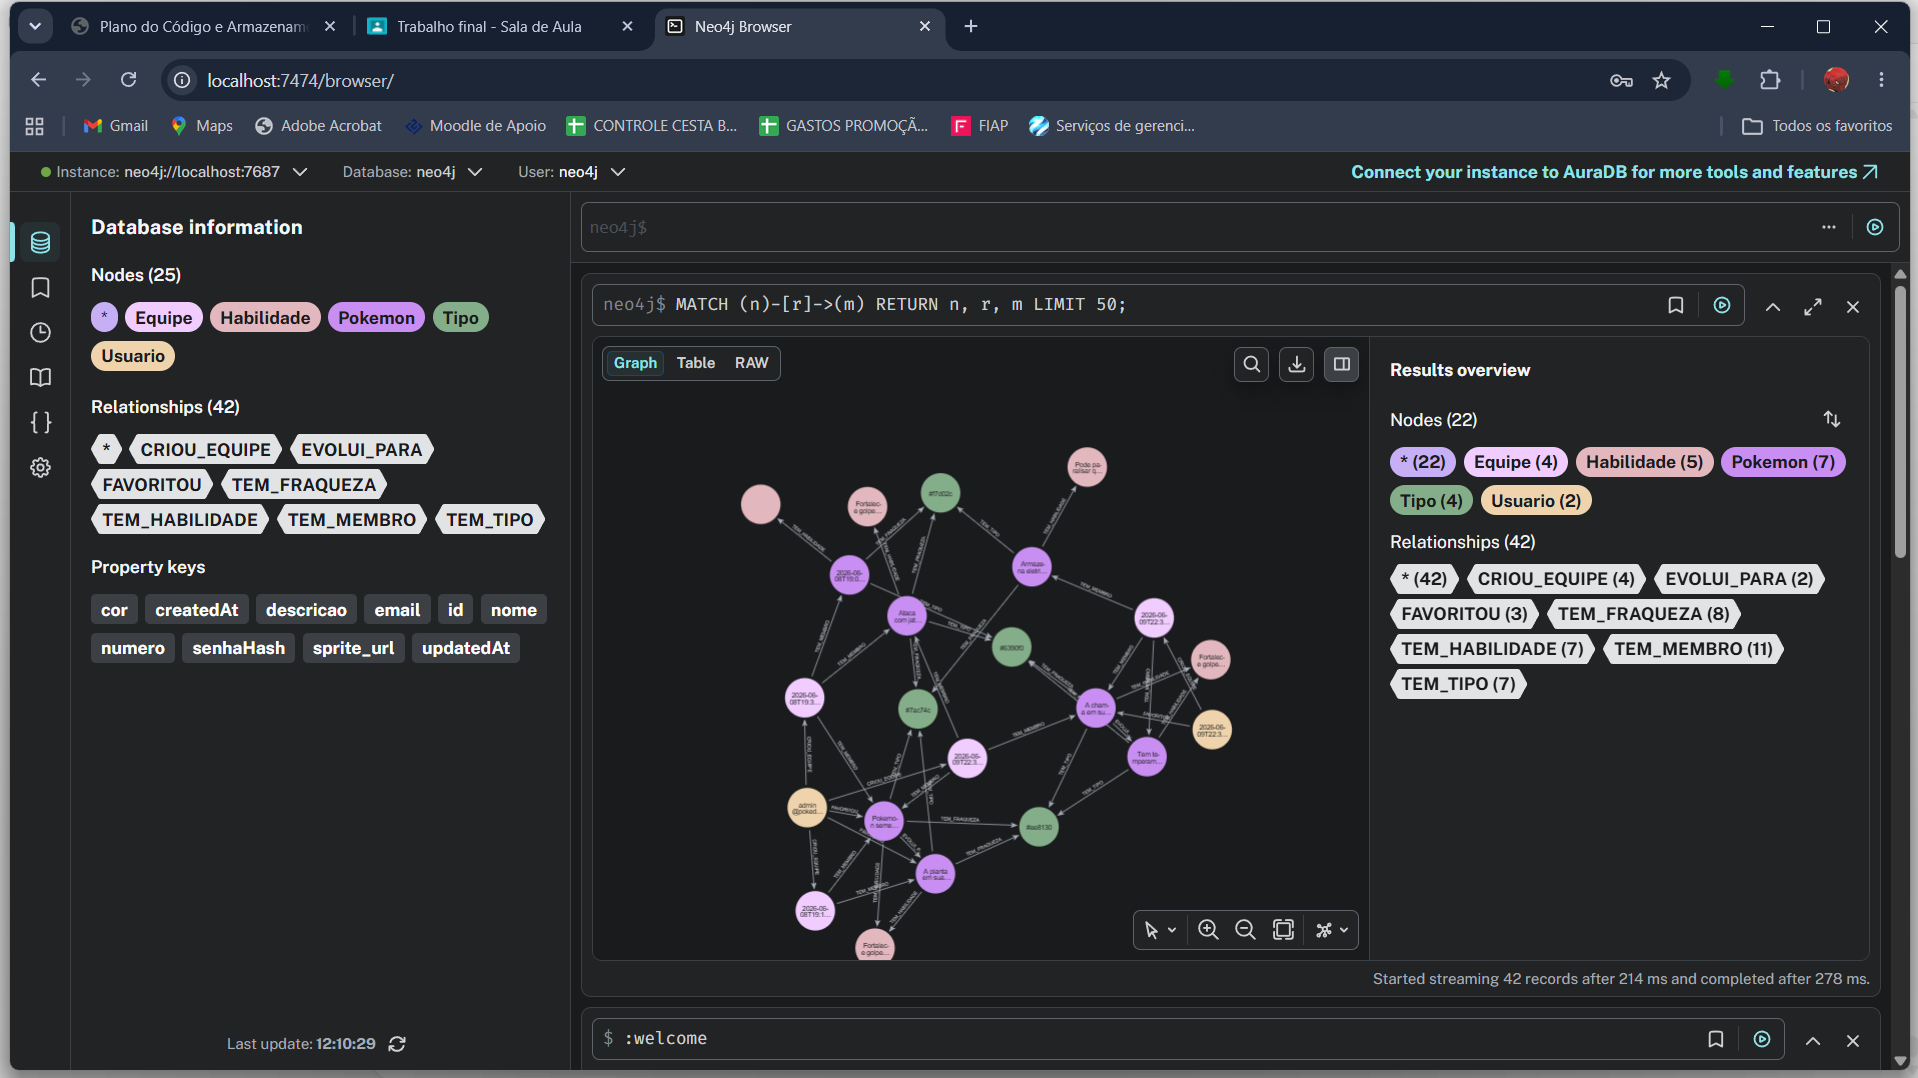
\includegraphics[width=.95\textwidth]{figuras/neo4j-grafo.png}
\caption{Visualização de nós e relacionamentos no Neo4j Browser.}
\label{fig:neo4j}
\end{figure}

Os testes realizados confirmaram o funcionamento das rotas principais. O login retornou token JWT, as rotas protegidas aceitaram requisições com cabeçalho de autorização, e as operações temporárias de criação, atualização e remoção de Pokémon e Tipo foram executadas com sucesso.

\begin{table}[H]
\centering
\caption{Resumo dos testes funcionais realizados.}
\label{tab:testes}
\begin{tabular}{p{4cm}p{9cm}}
\toprule
\textbf{Teste} & \textbf{Resultado observado}\\
\midrule
GET /health & Retornou mensagem de funcionamento da API.\\
GET /pokemons & Retornou a lista inicial de Pokémon.\\
POST /auth/login & Retornou usuário autenticado e token JWT.\\
CRUD de Pokémon & Permitiu criar, atualizar e remover registro temporário.\\
CRUD de Tipo & Permitiu criar, atualizar e remover tipo temporário.\\
Neo4j Browser & Exibiu nós e relacionamentos do grafo.\\
Docker & Containers da aplicação e do Neo4j permaneceram ativos.\\
\bottomrule
\end{tabular}
\end{table}

\begin{figure}[H]
\centering
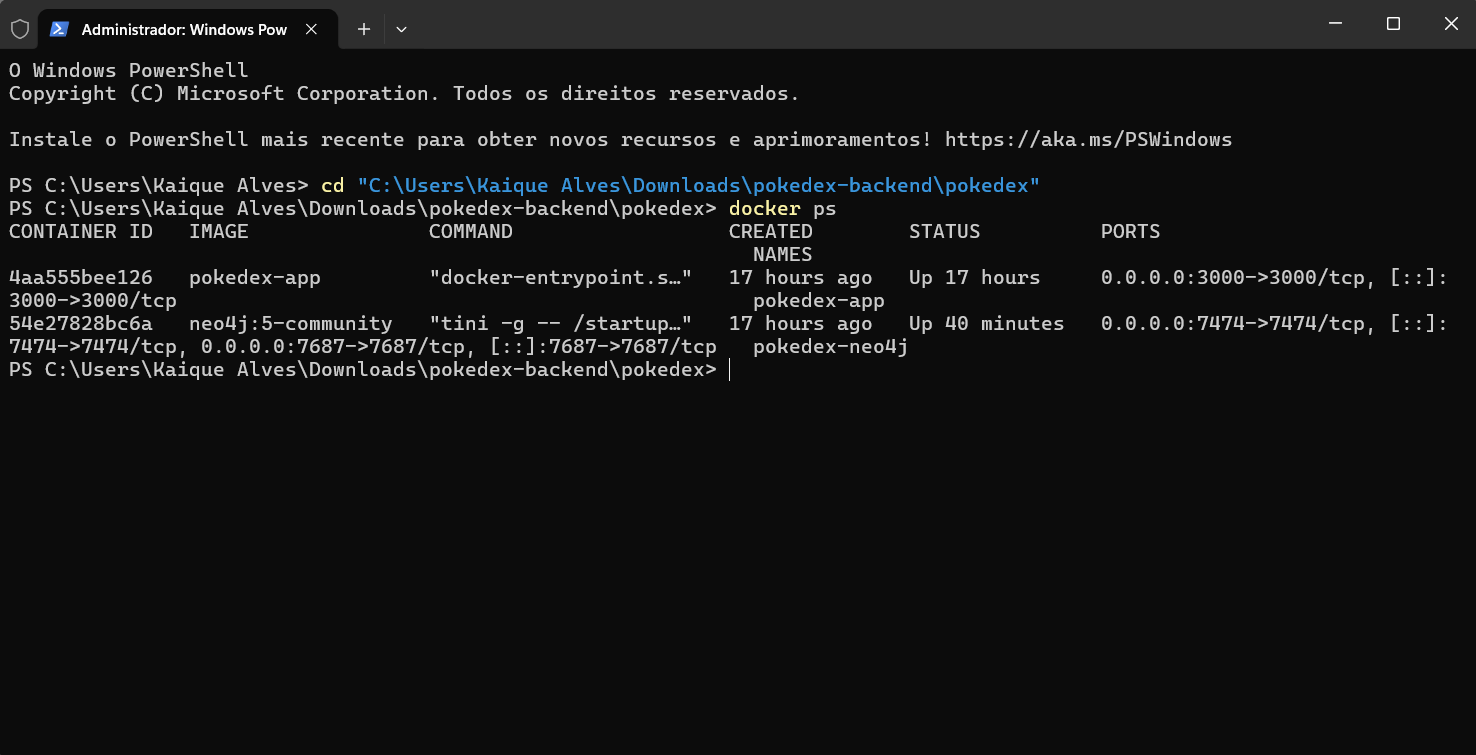
\includegraphics[width=.95\textwidth]{figuras/docker-ps.png}
\caption{Containers Docker da aplicação e do Neo4j em execução.}
\label{fig:dockerps}
\end{figure}

\section{Discussão}

O uso de grafo mostrou-se adequado para o domínio da Pokedex porque os relacionamentos são parte essencial do problema. A representação por nós e arestas simplificou a compreensão da modelagem e tornou visíveis conexões que, em um modelo tabular, dependeriam de várias tabelas intermediárias.

Outro ponto relevante foi a separação entre front-end e back-end. O front-end concentra a interação do usuário, enquanto o back-end centraliza regras de negócio, segurança e persistência. Essa divisão favorece manutenção e permite evoluir a API sem reescrever toda a interface.

A autenticação com JWT e bcrypt também contribuiu para a segurança mínima da aplicação. O bcrypt impede o armazenamento de senhas em texto puro, enquanto o JWT permite proteger rotas sem manter sessão no servidor. Entretanto, em um ambiente de produção real, seriam necessários cuidados adicionais, como uso de HTTPS, política de renovação de tokens, proteção contra ataques de força bruta e variáveis de ambiente com segredos mais robustos.

Em relação ao Docker, a conteinerização facilitou a execução do ambiente, principalmente por separar aplicação e banco em serviços independentes. O uso de volumes para o Neo4j contribui para persistência dos dados, enquanto a rede Docker personalizada permite comunicação entre os containers pelo nome do serviço.

\section{Conclusão e Trabalhos Futuros}

Este artigo apresentou o desenvolvimento de uma Pokedex em Grafos com front-end em HTML, CSS e JavaScript puro, API REST em Node.js com Express, autenticação JWT, senhas com bcrypt e persistência em Neo4j. O sistema atende aos requisitos de uma aplicação web completa ao integrar cadastro, login, recursos principais, CRUD, validações, logs, tratamento centralizado de erros e consumo da API pelo front-end.

Os resultados demonstram que a modelagem em grafo é apropriada para representar o domínio Pokémon, pois permite tratar relações como favoritos, equipes, tipos, fraquezas, habilidades e evoluções de forma direta. Além disso, o ambiente com Docker facilita a execução da aplicação e do banco de dados.

Como trabalhos futuros, propõe-se ampliar o catálogo de Pokémon, adicionar edição completa de equipes, incluir permissões por perfil de usuário, criar testes automatizados de API, implementar paginação e busca avançada, melhorar a visualização gráfica no front-end e disponibilizar a aplicação em ambiente de nuvem com banco persistente gerenciado.

\bibliographystyle{sbc}
\bibliography{referencias}

\end{document}
